% cd /storage/emulated/0/Documents/documents/latex/1920/Grade-8/3rd/theorems-on-perpendicular-lines/&& pdflatex hand-theorems-on-perpendicular-lines.tex && divide 2x2 hand-theorems-on-perpendicular-lines.pdf


\documentclass[handout]{beamer} 

\usepackage{pgfpages} 
\mode<handout>{%
\pgfpagesuselayout{4 on 1}[%letterpaper, 
legalpaper,% landscape, 
border shrink=1mm] 
}

\usepackage{xcolor}
\usepackage{anyfontsize}
\usepackage{enumitem}
\usepackage{multicol}
\usepackage{amsmath, makecell}
\usepackage{tabularx} 
\usepackage{gensymb}
\usepackage{wasysym} %for checked symbol 
\usepackage{multirow}
\usepackage{graphicx, tipa}
\usepackage{tikz}
\usetikzlibrary{angles,quotes}
\usepackage{pgfplots} 
\usetikzlibrary{calc}
\pgfplotsset{compat=newest}
\usetikzlibrary{arrows.meta}
\usetikzlibrary{intersections}
\usetikzlibrary{decorations.pathreplacing}
\usepackage{flafter}
%\usepackage{fourier} 
\usepackage{amsmath,amssymb,cancel,units}
\usepackage{microtype} % nicer output 
\usepackage{hfoldsty} % nicer output 
\usepackage{fixltx2e} 
\usepackage{mathptmx}
\usepackage{numprint}
\usepackage[T1]{fontenc}
\usepackage[utf8]{inputenc} 
\usepackage{stackengine} %to define \pesos 
\usepackage{lmodern} %scalable font
\usepackage{booktabs}
\usepackage{array}


\pagenumbering{gobble}
%\linespread{0.9}
\newcommand{\vspce}{\vspace{0.75ex}}

\newcommand{\hspce}{\hspace{0.5em}}

\newcommand{\blank}{\underline{\hspace{2em}}}%{\rule{1em}{0.15ex}}

\newcommand{\arc}[1]{{% 
\setbox9=\hbox{#1}% 
\ooalign{\resizebox{\wd9}{\height}{\texttoptiebar{\phantom{A}}}\cr#1}}}


\newcommand\pesos{\stackengine{-1.4ex}{P}{\stackengine{-1.25ex}{$-$}{$-$}{O}{c}{F}{F}{S}}{O}{c}{F}{T}{S}} 


\renewcommand\theadalign{bc} 

\renewcommand\theadfont{\bfseries} 

\renewcommand\theadgape{\Gape[4pt]} 

\renewcommand\cellgape{\Gape[4pt]} 

\pagenumbering{gobble}

\newcolumntype{Y}{>{\centering\arraybackslash}X} %for tabularx

\newcolumntype{R}{>{\raggedleft\arraybackslash}X} %for tabularx

\newcolumntype{Z}{>{\raggedleft\arraybackslash}X} %for tabularx

\newcolumntype{L}{>{\raggedright\arraybackslash}X} %for tabularx

\newcolumntype{A}[1]{>{\raggedright\arraybackslash}p{#1}} %for longtable LEFT

\newcolumntype{C}[1]{>{\centering\arraybackslash}p{#1}} %for longtable CENTER

\newcolumntype{B}[1]{>{\raggedleft\arraybackslash}p{#1}} %for longtable RIGHT 
 
\renewcommand{\tabularxcolumn}[1]{>{\small}m{#1}}

\newcolumntype{N}[1]{>{\raggedleft}p{#1}} %for tabular left 

\newcolumntype{M}[1]{>{\raggedright\arraybackslash}p{#1}} %for tabular right 

\newcommand{\myaxis}{xticklabels={}, 
yticklabels={}, 
ymin=-10, ymax=10,
xmin=-10, xmax=10,
axis lines = center, 
inner axis line style={Latex-Latex,very thick}, 
grid=both,
minor tick num=4, 
tick align=inside} % grid without labels, origin at the center, 10 units from origin

\newcommand{\axisfive}{xticklabels={}, 
yticklabels={}, 
ymin=-5, ymax=5,
xmin=-5, xmax=5,
axis lines = center, 
inner axis line style={Latex-Latex,very thick}, 
grid=both,
minor tick num=1, 
tick align=inside} % grid with labels, origin at the center, 5 units from origin 

\newcommand \redcheck {{\color{red}\checkmark}}



%\setbeamertemplate{itemize items}{\textbullet} 
%\useinnertheme{circles} 

%\newcommand{\vertadjust}{\vspace*{-1.5in}} % for letterpaper
%\newcommand{\vertadjustb}{\vspace*{-1.5in}} % for letterpaper
\newcommand{\vertadjust}{\vspace*{-2.5in}} % for legalpaper
\newcommand{\vertadjustb}{\vspace*{-2.5in}} % for legalpaper

\def\lenA{1.3cm}
\def\lenB{1.2cm}
\def\leninnersep{\lenA}

\begin{document} 

% frame 1
\vertadjust
\begin{frame} 
\begin{center}
\textbf{Theorems on Perpendicular Lines}
\end{center}

\vspace*{1ex}

%\begin{center}
%\vspace*{-2ex}
\scalebox{0.9}{
\noindent\begin{minipage}{\textwidth}
{

%\end{center} 
\textbf{Perpendicular Lines:} two lines that meet to form congruent adjacent angles

\vspce 

\textbf{Parallel Lines:} lines that lie in the same plane and have no point in common

\vspce 

\textbf{Theorems on Perpendicular Lines:}
\begin{enumerate}[label = \arabic*. ]
%1
\item If two lines are perpendicular, then they form four right angles.
%2
\item If two lines meet to form a right angle, the lines are perpendicular.
%3
\item In a plane, through a given point of a line, there is exactly one line perpendicular to the line.
\end{enumerate}   
}
\end{minipage}}




 %\\
%\input{hand-theorems-on-perpendicular-lines-input1}
\textbf{Practice Exercises}

\vspce

The adjoining figure consists of 3 coplanar lines passing through $O$ with $\overline{AB} \perp \overline{CD}$. Determine each statement as true or false.

%\begin{center}
%\vspace*{2ex}
%\scalebox{1}{
%\noindent\begin{minipage}{\textwidth}
{\begin{enumerate}[label = \arabic*. ]
%\begin{multicols}{2}
%1
\item	$m\angle{AOC}=90\degree$ 
\item	$m\angle{FOD}= m\angle{AOD} - m\angle{AOF}$ 
\item	$\angle{COF}$ is an acute angle
\item	$\overleftrightarrow{EF} \perp \overleftrightarrow{CD}$ 
\item	$\overrightarrow{OC}$ and $\overrightarrow{OF}$ are opposite rays 
\item	$\angle{AOF}$ and $\angle{AOD}$ are adjacent angles
\item	$\angle{AOD}$ is a right angle
\item	$\angle{AOC}$ and $\angle{AOD}$ are congruent\\ adjacent supplementary angles.
\item	The exterior sides of $\angle{AOF}$ and $\angle{FOD}$ lie in perpendicular lines.
\item	$\overrightarrow{OB} \perp \overrightarrow{OD} $
%\end{multicols} 
\end{enumerate}}
%\end{minipage}}
%\end{center}  

\vspace*{-14.5em}\hspace*{18em}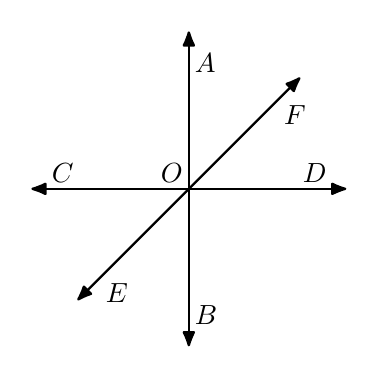
\begin{tikzpicture}

\coordinate (O) at (0,0);

\node[anchor=south east, inner sep=2pt, rotate=0] (O-label) at (O) {$O$}; 

\foreach \ang/\label/\dir in {0/D/south,45/F/north west,90/A/west,180/C/south,225/E/north west,270/B/west} {

\coordinate (\label) at ($(O) + (\ang:2cm)$); 

\draw[line width=0.3mm, ->, >={Latex[round]}] (O) -- (\label);  

\node[anchor=\dir, inner sep=2pt, rotate=0] (label-\label) at ($(O)+ (\ang:1.6cm)$) {$\label$};
}

\end{tikzpicture} 
 
\vspace*{2em}


     






%\input{ps-theorems-on-perpendicular-lines-input2}
\vspace*{1ex}
\textbf{Problem Set}

\vspce

The adjoining figure consists of 3 coplanar lines passing through $O$ with $\overline{AL} \perp \overline{UB}$. Determine each statement as true or false.

%\begin{center}
%\vspace*{2ex}
%\scalebox{1}{
%\noindent\begin{minipage}{\textwidth}
{\begin{enumerate}[label = \arabic*. ]
%\begin{multicols}{2}
%1
\item	$m\angle{AOB}=90\degree$ 
\item	$m\angle{KOU}= m\angle{AOU} - m\angle{AOK}$ 
\item	$\angle{KOB}$ is an acute angle
\item	$\overleftrightarrow{KW} \perp \overleftrightarrow{UB}$ 
\item	$\overrightarrow{OB}$ and $\overrightarrow{OK}$ are opposite rays 
\item	$\angle{AOK}$ and $\angle{AOU}$ are adjacent angles
\item	$\angle{AOU}$ is a right angle
\item	$\angle{AOB}$ and $\angle{AOU}$ are congruent\\ adjacent supplementary angles.
\item	The exterior sides of $\angle{AOK}$ and $\angle{KOU}$ lie in perpendicular lines.
\item	$\overrightarrow{OL} \perp \overrightarrow{OU} $
%\end{multicols} 
\end{enumerate}}
%\end{minipage}}
%\end{center}  

\vspace*{-14.5em}\hspace*{18em}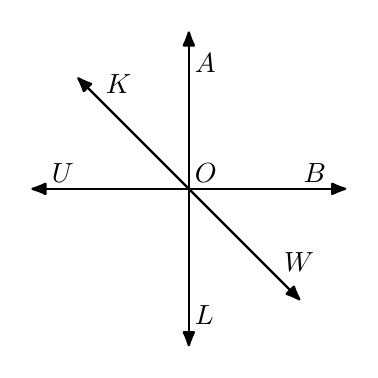
\begin{tikzpicture}

\coordinate (O) at (0,0);

\node[anchor=south west, inner sep=2pt, rotate=0] (O-label) at (O) {$O$}; 

\foreach \ang/\label/\dir in {0/B/south,90/A/west,135/K/south west,180/U/south,270/L/west,315/W/south west} {

\coordinate (\label) at ($(O) + (\ang:2cm)$); 

\draw[line width=0.3mm, ->, >={Latex[round]}] (O) -- (\label);  

\node[anchor=\dir, inner sep=2pt, rotate=0] (label-\label) at ($(O)+ (\ang:1.6cm)$) {$\label$};
}

\end{tikzpicture} 
 
\vspace*{2em}


     






\end{frame}

% frame 2
\vertadjust
\begin{frame} 
\begin{center}
\textbf{Theorems on Perpendicular Lines}
\end{center}

\vspace*{1ex}

%\begin{center}
%\vspace*{-2ex}
\scalebox{0.9}{
\noindent\begin{minipage}{\textwidth}
{

%\end{center} 
\textbf{Perpendicular Lines:} two lines that meet to form congruent adjacent angles

\vspce 

\textbf{Parallel Lines:} lines that lie in the same plane and have no point in common

\vspce 

\textbf{Theorems on Perpendicular Lines:}
\begin{enumerate}[label = \arabic*. ]
%1
\item If two lines are perpendicular, then they form four right angles.
%2
\item If two lines meet to form a right angle, the lines are perpendicular.
%3
\item In a plane, through a given point of a line, there is exactly one line perpendicular to the line.
\end{enumerate}   
}
\end{minipage}}




% \\
%\input{vs-theorems-on-perpendicular-lines-input2}
\textbf{Practice Exercises}

\vspce

The adjoining figure consists of 3 coplanar lines passing through $O$ with $\overline{AB} \perp \overline{CD}$. Determine each statement as true or false.

%\begin{center}
%\vspace*{2ex}
%\scalebox{1}{
%\noindent\begin{minipage}{\textwidth}
{\begin{enumerate}[label = \arabic*. ]
%\begin{multicols}{2}
%1
\item	$m\angle{AOC}=90\degree$ 
\item	$m\angle{FOD}= m\angle{AOD} - m\angle{AOF}$ 
\item	$\angle{COF}$ is an acute angle
\item	$\overleftrightarrow{EF} \perp \overleftrightarrow{CD}$ 
\item	$\overrightarrow{OC}$ and $\overrightarrow{OF}$ are opposite rays 
\item	$\angle{AOF}$ and $\angle{AOD}$ are adjacent angles
\item	$\angle{AOD}$ is a right angle
\item	$\angle{AOC}$ and $\angle{AOD}$ are congruent\\ adjacent supplementary angles.
\item	The exterior sides of $\angle{AOF}$ and $\angle{FOD}$ lie in perpendicular lines.
\item	$\overrightarrow{OB} \perp \overrightarrow{OD} $
%\end{multicols} 
\end{enumerate}}
%\end{minipage}}
%\end{center}  

\vspace*{-14.5em}\hspace*{18em}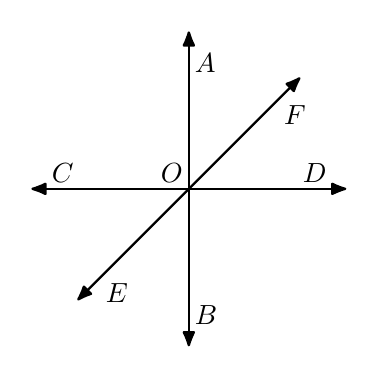
\begin{tikzpicture}

\coordinate (O) at (0,0);

\node[anchor=south east, inner sep=2pt, rotate=0] (O-label) at (O) {$O$}; 

\foreach \ang/\label/\dir in {0/D/south,45/F/north west,90/A/west,180/C/south,225/E/north west,270/B/west} {

\coordinate (\label) at ($(O) + (\ang:2cm)$); 

\draw[line width=0.3mm, ->, >={Latex[round]}] (O) -- (\label);  

\node[anchor=\dir, inner sep=2pt, rotate=0] (label-\label) at ($(O)+ (\ang:1.6cm)$) {$\label$};
}

\end{tikzpicture} 
 
\vspace*{2em}


     






%\input{ps-theorems-on-perpendicular-lines-input2}
\vspace*{1ex}
\textbf{Problem Set}

\vspce

The adjoining figure consists of 3 coplanar lines passing through $O$ with $\overline{AL} \perp \overline{UB}$. Determine each statement as true or false.

%\begin{center}
%\vspace*{2ex}
%\scalebox{1}{
%\noindent\begin{minipage}{\textwidth}
{\begin{enumerate}[label = \arabic*. ]
%\begin{multicols}{2}
%1
\item	$m\angle{AOB}=90\degree$ 
\item	$m\angle{KOU}= m\angle{AOU} - m\angle{AOK}$ 
\item	$\angle{KOB}$ is an acute angle
\item	$\overleftrightarrow{KW} \perp \overleftrightarrow{UB}$ 
\item	$\overrightarrow{OB}$ and $\overrightarrow{OK}$ are opposite rays 
\item	$\angle{AOK}$ and $\angle{AOU}$ are adjacent angles
\item	$\angle{AOU}$ is a right angle
\item	$\angle{AOB}$ and $\angle{AOU}$ are congruent\\ adjacent supplementary angles.
\item	The exterior sides of $\angle{AOK}$ and $\angle{KOU}$ lie in perpendicular lines.
\item	$\overrightarrow{OL} \perp \overrightarrow{OU} $
%\end{multicols} 
\end{enumerate}}
%\end{minipage}}
%\end{center}  

\vspace*{-14.5em}\hspace*{18em}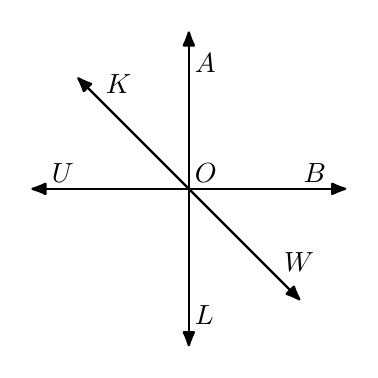
\begin{tikzpicture}

\coordinate (O) at (0,0);

\node[anchor=south west, inner sep=2pt, rotate=0] (O-label) at (O) {$O$}; 

\foreach \ang/\label/\dir in {0/B/south,90/A/west,135/K/south west,180/U/south,270/L/west,315/W/south west} {

\coordinate (\label) at ($(O) + (\ang:2cm)$); 

\draw[line width=0.3mm, ->, >={Latex[round]}] (O) -- (\label);  

\node[anchor=\dir, inner sep=2pt, rotate=0] (label-\label) at ($(O)+ (\ang:1.6cm)$) {$\label$};
}

\end{tikzpicture} 
 
\vspace*{2em}


     






\end{frame}

% frame 3
\vertadjustb
\begin{frame} 
\begin{center}
\textbf{Theorems on Perpendicular Lines}
\end{center}

\vspace*{1ex}

%\begin{center}
%\vspace*{-2ex}
\scalebox{0.9}{
\noindent\begin{minipage}{\textwidth}
{

%\end{center} 
\textbf{Perpendicular Lines:} two lines that meet to form congruent adjacent angles

\vspce 

\textbf{Parallel Lines:} lines that lie in the same plane and have no point in common

\vspce 

\textbf{Theorems on Perpendicular Lines:}
\begin{enumerate}[label = \arabic*. ]
%1
\item If two lines are perpendicular, then they form four right angles.
%2
\item If two lines meet to form a right angle, the lines are perpendicular.
%3
\item In a plane, through a given point of a line, there is exactly one line perpendicular to the line.
\end{enumerate}   
}
\end{minipage}}




 
\textbf{Practice Exercises}

\vspce

The adjoining figure consists of 3 coplanar lines passing through $O$ with $\overline{AB} \perp \overline{CD}$. Determine each statement as true or false.

%\begin{center}
%\vspace*{2ex}
%\scalebox{1}{
%\noindent\begin{minipage}{\textwidth}
{\begin{enumerate}[label = \arabic*. ]
%\begin{multicols}{2}
%1
\item	$m\angle{AOC}=90\degree$ 
\item	$m\angle{FOD}= m\angle{AOD} - m\angle{AOF}$ 
\item	$\angle{COF}$ is an acute angle
\item	$\overleftrightarrow{EF} \perp \overleftrightarrow{CD}$ 
\item	$\overrightarrow{OC}$ and $\overrightarrow{OF}$ are opposite rays 
\item	$\angle{AOF}$ and $\angle{AOD}$ are adjacent angles
\item	$\angle{AOD}$ is a right angle
\item	$\angle{AOC}$ and $\angle{AOD}$ are congruent\\ adjacent supplementary angles.
\item	The exterior sides of $\angle{AOF}$ and $\angle{FOD}$ lie in perpendicular lines.
\item	$\overrightarrow{OB} \perp \overrightarrow{OD} $
%\end{multicols} 
\end{enumerate}}
%\end{minipage}}
%\end{center}  

\vspace*{-14.5em}\hspace*{18em}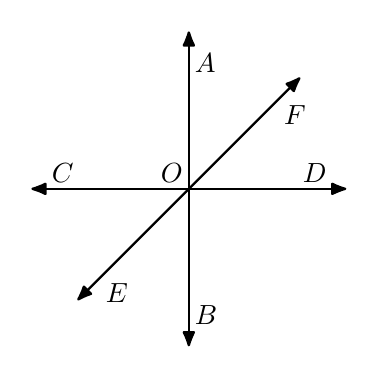
\begin{tikzpicture}

\coordinate (O) at (0,0);

\node[anchor=south east, inner sep=2pt, rotate=0] (O-label) at (O) {$O$}; 

\foreach \ang/\label/\dir in {0/D/south,45/F/north west,90/A/west,180/C/south,225/E/north west,270/B/west} {

\coordinate (\label) at ($(O) + (\ang:2cm)$); 

\draw[line width=0.3mm, ->, >={Latex[round]}] (O) -- (\label);  

\node[anchor=\dir, inner sep=2pt, rotate=0] (label-\label) at ($(O)+ (\ang:1.6cm)$) {$\label$};
}

\end{tikzpicture} 
 
\vspace*{2em}


     






%\input{ps-theorems-on-perpendicular-lines-input2}
\vspace*{1ex}
\textbf{Problem Set}

\vspce

The adjoining figure consists of 3 coplanar lines passing through $O$ with $\overline{AL} \perp \overline{UB}$. Determine each statement as true or false.

%\begin{center}
%\vspace*{2ex}
%\scalebox{1}{
%\noindent\begin{minipage}{\textwidth}
{\begin{enumerate}[label = \arabic*. ]
%\begin{multicols}{2}
%1
\item	$m\angle{AOB}=90\degree$ 
\item	$m\angle{KOU}= m\angle{AOU} - m\angle{AOK}$ 
\item	$\angle{KOB}$ is an acute angle
\item	$\overleftrightarrow{KW} \perp \overleftrightarrow{UB}$ 
\item	$\overrightarrow{OB}$ and $\overrightarrow{OK}$ are opposite rays 
\item	$\angle{AOK}$ and $\angle{AOU}$ are adjacent angles
\item	$\angle{AOU}$ is a right angle
\item	$\angle{AOB}$ and $\angle{AOU}$ are congruent\\ adjacent supplementary angles.
\item	The exterior sides of $\angle{AOK}$ and $\angle{KOU}$ lie in perpendicular lines.
\item	$\overrightarrow{OL} \perp \overrightarrow{OU} $
%\end{multicols} 
\end{enumerate}}
%\end{minipage}}
%\end{center}  

\vspace*{-14.5em}\hspace*{18em}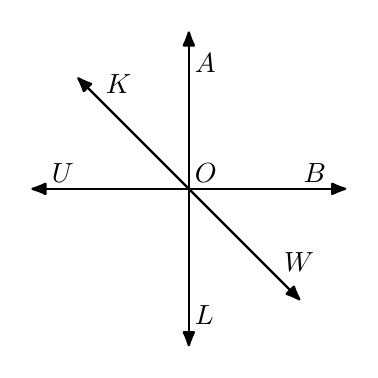
\begin{tikzpicture}

\coordinate (O) at (0,0);

\node[anchor=south west, inner sep=2pt, rotate=0] (O-label) at (O) {$O$}; 

\foreach \ang/\label/\dir in {0/B/south,90/A/west,135/K/south west,180/U/south,270/L/west,315/W/south west} {

\coordinate (\label) at ($(O) + (\ang:2cm)$); 

\draw[line width=0.3mm, ->, >={Latex[round]}] (O) -- (\label);  

\node[anchor=\dir, inner sep=2pt, rotate=0] (label-\label) at ($(O)+ (\ang:1.6cm)$) {$\label$};
}

\end{tikzpicture} 
 
\vspace*{2em}


     






\end{frame}

% frame 4
\vertadjustb
\begin{frame} 
\begin{center}
\textbf{Theorems on Perpendicular Lines}
\end{center}

\vspace*{1ex}

%\begin{center}
%\vspace*{-2ex}
\scalebox{0.9}{
\noindent\begin{minipage}{\textwidth}
{

%\end{center} 
\textbf{Perpendicular Lines:} two lines that meet to form congruent adjacent angles

\vspce 

\textbf{Parallel Lines:} lines that lie in the same plane and have no point in common

\vspce 

\textbf{Theorems on Perpendicular Lines:}
\begin{enumerate}[label = \arabic*. ]
%1
\item If two lines are perpendicular, then they form four right angles.
%2
\item If two lines meet to form a right angle, the lines are perpendicular.
%3
\item In a plane, through a given point of a line, there is exactly one line perpendicular to the line.
\end{enumerate}   
}
\end{minipage}}





%\input{vs-theorems-on-perpendicular-lines-input2}
\textbf{Practice Exercises}

\vspce

The adjoining figure consists of 3 coplanar lines passing through $O$ with $\overline{AB} \perp \overline{CD}$. Determine each statement as true or false.

%\begin{center}
%\vspace*{2ex}
%\scalebox{1}{
%\noindent\begin{minipage}{\textwidth}
{\begin{enumerate}[label = \arabic*. ]
%\begin{multicols}{2}
%1
\item	$m\angle{AOC}=90\degree$ 
\item	$m\angle{FOD}= m\angle{AOD} - m\angle{AOF}$ 
\item	$\angle{COF}$ is an acute angle
\item	$\overleftrightarrow{EF} \perp \overleftrightarrow{CD}$ 
\item	$\overrightarrow{OC}$ and $\overrightarrow{OF}$ are opposite rays 
\item	$\angle{AOF}$ and $\angle{AOD}$ are adjacent angles
\item	$\angle{AOD}$ is a right angle
\item	$\angle{AOC}$ and $\angle{AOD}$ are congruent\\ adjacent supplementary angles.
\item	The exterior sides of $\angle{AOF}$ and $\angle{FOD}$ lie in perpendicular lines.
\item	$\overrightarrow{OB} \perp \overrightarrow{OD} $
%\end{multicols} 
\end{enumerate}}
%\end{minipage}}
%\end{center}  

\vspace*{-14.5em}\hspace*{18em}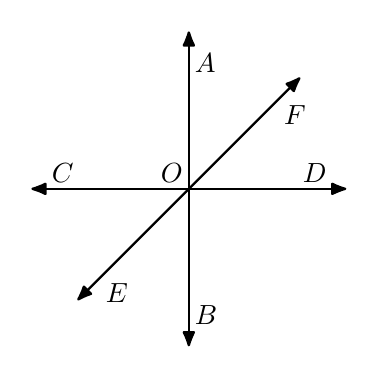
\begin{tikzpicture}

\coordinate (O) at (0,0);

\node[anchor=south east, inner sep=2pt, rotate=0] (O-label) at (O) {$O$}; 

\foreach \ang/\label/\dir in {0/D/south,45/F/north west,90/A/west,180/C/south,225/E/north west,270/B/west} {

\coordinate (\label) at ($(O) + (\ang:2cm)$); 

\draw[line width=0.3mm, ->, >={Latex[round]}] (O) -- (\label);  

\node[anchor=\dir, inner sep=2pt, rotate=0] (label-\label) at ($(O)+ (\ang:1.6cm)$) {$\label$};
}

\end{tikzpicture} 
 
\vspace*{2em}


     






%\input{ps-theorems-on-perpendicular-lines-input2}
\vspace*{1ex}
\textbf{Problem Set}

\vspce

The adjoining figure consists of 3 coplanar lines passing through $O$ with $\overline{AL} \perp \overline{UB}$. Determine each statement as true or false.

%\begin{center}
%\vspace*{2ex}
%\scalebox{1}{
%\noindent\begin{minipage}{\textwidth}
{\begin{enumerate}[label = \arabic*. ]
%\begin{multicols}{2}
%1
\item	$m\angle{AOB}=90\degree$ 
\item	$m\angle{KOU}= m\angle{AOU} - m\angle{AOK}$ 
\item	$\angle{KOB}$ is an acute angle
\item	$\overleftrightarrow{KW} \perp \overleftrightarrow{UB}$ 
\item	$\overrightarrow{OB}$ and $\overrightarrow{OK}$ are opposite rays 
\item	$\angle{AOK}$ and $\angle{AOU}$ are adjacent angles
\item	$\angle{AOU}$ is a right angle
\item	$\angle{AOB}$ and $\angle{AOU}$ are congruent\\ adjacent supplementary angles.
\item	The exterior sides of $\angle{AOK}$ and $\angle{KOU}$ lie in perpendicular lines.
\item	$\overrightarrow{OL} \perp \overrightarrow{OU} $
%\end{multicols} 
\end{enumerate}}
%\end{minipage}}
%\end{center}  

\vspace*{-14.5em}\hspace*{18em}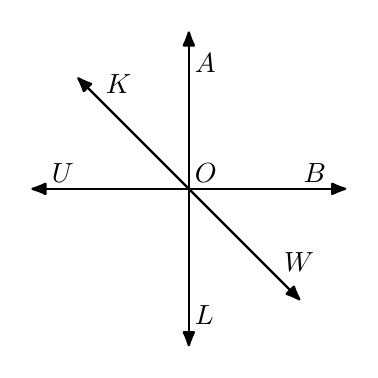
\begin{tikzpicture}

\coordinate (O) at (0,0);

\node[anchor=south west, inner sep=2pt, rotate=0] (O-label) at (O) {$O$}; 

\foreach \ang/\label/\dir in {0/B/south,90/A/west,135/K/south west,180/U/south,270/L/west,315/W/south west} {

\coordinate (\label) at ($(O) + (\ang:2cm)$); 

\draw[line width=0.3mm, ->, >={Latex[round]}] (O) -- (\label);  

\node[anchor=\dir, inner sep=2pt, rotate=0] (label-\label) at ($(O)+ (\ang:1.6cm)$) {$\label$};
}

\end{tikzpicture} 
 
\vspace*{2em}


     







\end{frame}

\end{document}

